\documentclass[../main.tex]{subfiles}
\begin{document}

\chapter{Iterative Methods}
\begin{center}
\textbf{CHAPTER OBJECTIVES}
\end{center}
The primary objective of this chapter is to acquaint you with iterative methods for
solving simultaneous equations. Specific objectives and topics covered are
\begin{itemize}
\item Understanding the difference between the Gauss-Seidel and Jacobi methods.
\item Knowing how to assess diagonal dominance and knowing what it means.
\item Recognizing how relaxation can be used to improve the convergence of iterative
methods.
\item Knowing how to implement the power method to evaluate the largest and smallest eigenvalues and their respective eigenvectors.Understanding how to solve systems of nonlinear equations with successive
substitution and Newton-Raphson.
\end{itemize}
terative or approximate methods provide an alternative to the elimination methods
described to this point. Such approaches are similar to the techniques we developed to
obtain the roots of a single equation in Chaps. 5 and 6. Those approaches consisted of
guessing a value and then using a systematic method to obtain a refined estimate of the root.
Because the present part of the book deals with a similar problem obtaining the values
that simultaneously satisfy a set of equations we might suspect that such approximate methods could be useful in this context.
In this chapter, we will present approaches for
solving both linear and nonlinear simultaneous equations.

\textbf{12.1 LINEAR SYSTEMS: GAUSS-SEIDEL}

The Gauss-Seidel method is the most commonly used iterative method for solving linear
algebraic equations. Assume that we are given a set of n equations:
\begin{equation}
[A]\{x\}=\{b\}
\end{equation}

Suppose that for conciseness we limit ourselves to a 3 × 3 set of equations. If the diagonal
elements are all nonzero, the first equation can be solved for x1, the second for $x_{2}$, and the third for $x_{3}$ to yield

\begin{equation}
x_{1}^{j}=\frac{b_{1}-a_{12}x_{2}^{j-1}-a_{13}x_{3}^{j-1}}{a_{11}}\tag{12.1a}
\end{equation}

\begin{equation}
x_{2}^{j}=\frac{b_{2}-a_{21}x_{1}^{j}-a_{23}x_{3}^{j-1}}{a_{22}}
\tag{12.1b}
\end{equation}

\begin{equation}
x_{3}^{j}=\frac{b_{3}-a_{31}x_{1}^{j}-a_{32}x_{2}^{j-1}}{a_{33}}
\tag{12.1c}
\end{equation}
'
where j and j - 1 are the present and previous iterations.
To start the solution process, initial guesses must be made for the x's. A simple approach is to assume that they are all zero. These zeros can be substituted into Eq. (12.1a),
which can be used to calculate a new value for $x_{1} = b_{1}/a_{11}$. Then we substitute this new
value of $x_{1}$ along with the previous guess of zero for $x_{3}$ into Eq. (12.1b) to compute a new
value for $x_{2}$. The process is repeated for Eq. (12.1c) to calculate a new estimate for $x_{3}$. Then
we return to the first equation and repeat the entire procedure until our solution converges
closely enough to the true values. Convergence can be checked using the criterion that for
all i,
\begin{equation}
\varepsilon _{a,i}=\begin{vmatrix}
\frac{x_{i}^{j}-x_{i}^{j-i}}{x_{i}^{j}}
\end{vmatrix}\times 100\%\leq \varepsilon_{s}
\end{equation}


\section*{EXAMPLE 12.1 Gauss-Seidel Method}

Problem Statement. Use the Gauss-Seidel method to obtain the solution for
\begin{equation}
3x_{1}-0.1x_{2}-0.2x_{3}=7.85
\end{equation}

\begin{equation}
0.1x_{1}+7x_{2}-0.3x_{3}=-19.3
\end{equation}

\begin{equation}
0.3x_{1}-0.2x_{2}+10x_{3}=71.4
\end{equation}

Note that the solutio is $x_{1}=3$, $x_{2}=-2.5$, anf $x_{3}=7$.

Solution. First, solve each of the equations for its unknown on the diagonal:

\begin{equation}
x_{1}=\frac{7.85+0.1x_{2}+0.2x_{3}}{3} \tag{E12.1.1}
\end{equation}

\begin{equation}
x_{2}=\frac{-19.3-0.1x_{1}+0.3x_{3}}{7} \tag{E12.1.2}
\end{equation}

\begin{equation}
x_{3}=\frac{71.4-0.3x_{1}+0.2x_{2}}{10}  \tag{E12.1.3}
\end{equation}

By assuming that $x_{2}$ and $x_{3}$ are zero, Eq. (E12.1.1) can be used to compute
\begin{equation}
x_{1}=\frac{7.85+0.1(0)+0.2(0)}{3}=2.616667
\end{equation}

This value, along with the assumed value of x3 = 0, can be substituted into Eq. (E12.1.2)
to calculate
\begin{equation}
x_{2}=\frac{-19.3-0.1(2.616667)+0.3(0)}{7}=-2.794524
\end{equation}

The first iteration is completed by substituting the calculated values for $x_{1}$ and $x_{2}$ into
Eq. (E12.1.3) to yield

\begin{equation}
x_{3}=\frac{71.4-0.3(2.616667)+0.2(-2.794524)}{10}=7.005610
\end{equation}

For the second iteration, the same process is repeated to compute

\begin{equation}
x_{1}=\frac{7.85+0.1(2.794524)+0.2(7.005610)}{3}=2.990557
\end{equation}

\begin{equation}
x_{2}=\frac{-19.3-0.1(2.990557)+03.(7.005610)}{7}=-2.499625
\end{equation}

\begin{equation}
x_{3}=\frac{71.4-0.3(2.990557)+02.(-2.499625)}{10}=7.000291
\end{equation}

The method is, therefore, converging on the true solution. Additional iterations could be
applied to improve the answers. However, in an actual problem, we would not know the
true answer a priori. Consequently, Eq. (12.2) provides a means to estimate the error. For
example, for $x_{1}$:

\begin{equation}
\varepsilon _{a,1}=\begin{vmatrix}
\frac{2.990557-2.616667}{2.990557}
\end{vmatrix}\times 100\%=12.5\%
\end{equation}

For $x_{2}$ and $x_{3}$, the error estimates are $\varepsilon_{a,2}=11.8\%$ and $\varepsilon_{a,3}=0.076\%$. Note that, as was
the case when determining roots of a single equation, formulations such as Eq. (12.2) usually provide a conservative appraisal of convergence. Thus, when they are met, they ensure that the result is known to at least the tolerance specified by $\varepsilon_{s}$.


As each new x value is computed for the Gauss-Seidel method, it is immediately used
in the next equation to determine another x value. Thus, if the solution is converging, the
best available estimates will be employed. An alternative approach, called Jacobi iteration,
utilizes a somewhat different tactic. Rather than using the latest available x's,
this technique uses Eq. (12.1) to compute a set of new x's on the basis of a set of old x's. Thus, as
new values are generated, they are not immediately used but rather are retained for the next
iteration.
The difference between the Gauss-Seidel method and Jacobi iteration is depicted in
Fig. 12.1. Although there are certain cases where the Jacobi method is useful, Gauss-Seidel's
utilization of the best available estimates usually makes it the method of preference.


\begin{figure}[H]
		\centering
		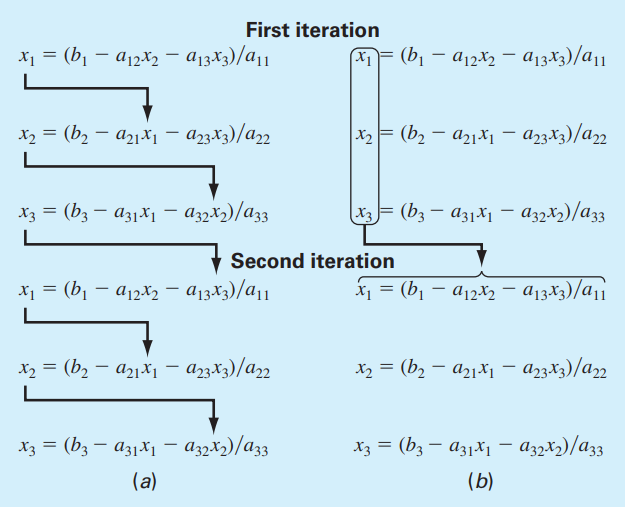
\includegraphics[width=0.75\textwidth]{fig_12_21}
	   \caption{\textsf{a) Graphical depiction of the difference between (a) the Gauss-Seidel and (b) the Jacobi iterative
methods for solving simultaneous linear algebraic equations.}}
	   \label{fig:fig_12_21}
\end{figure}


\section*{12.1.1 Convergence and Diagonal Dominance}

Note that the Gauss-Seidel method is similar in spirit to the technique of simple fixed-point
iteration that was used in Section 6.1 to solve for the roots of a single equation. Recall that
simple fixed-point iteration was sometimes nonconvergent. That is, as the iterations progressed, the answer moved farther and farther from the correct result.
Although the Gauss-Seidel method can also diverge, because it is designed for linear
systems, its ability to converge is much more predictable than for fixed-point iteration of
nonlinear equations. It can be shown that if the following condition holds, Gauss-Seidel
will converge:

\begin{equation}
\begin{vmatrix}
a_{ii}
\end{vmatrix}
> \sum_{\begin{matrix}
j=1\\
j\neq i
\end{matrix}}^{n} \begin{vmatrix}
a_{ij}
\end{vmatrix} \tag{12.3}
\end{equation}

That is, the absolute value of the diagonal coefficient in each of the equations must be
larger than the sum of the absolute values of the other coefficients in the equation. Such
systems are said to be diagonally dominant. This criterion is sufficient but not necessary
for convergence. That is, although the method may sometimes work if Eq. (12.3) is not
met, convergence is guaranteed if the condition is satisfied. Fortunately, many engineering and scientific problems of practical importance fulfill this requirement. Therefore,
Gauss-Seidel represents a feasible approach to solve many problems in engineering and
science.

\section*{12.1.2 MATLAB M-file: GaussSeidel}

Before developing an algorithm, let us first recast Gauss-Seidel in a form that is compatible with MATLAB's ability to perform matrix operations. This is done by expressing
Eq. (12.1) as

\begin{equation}
x_{1}^{new}=\frac{b_{1}}{a_{11}}
-\frac{a_{12}}{a_{11}}x_{2}^{old}-\frac{a_{13}}{a_{11}}x_{13}^{old}
\end{equation}

\begin{equation}
x_{12}^{new}=\frac{b_{2}}{a_{22}}-\frac{a_{21}}{a_{22}}x_{1}^{new}
-\frac{a_{23}}{a_{23}}x_{3}^{old}
\end{equation}

\begin{equation}
x_{3}^{new}= \frac{b_{3}}{a_{33}}-\frac{a_{31}}{a_{33}}x_{1}^{new}-\frac{a_{22}}{a_{33}}x_{2}^{new}
\end{equation}

Notice that the solution can be expressed concisely in matrix form as
\begin{equation}
\{x\}=\{d\}-[C]\{x\}
\tag{12.4}
\end{equation}

where

\begin{equation}
\{d\}=\begin{Bmatrix}
b_{1}/a{11}\\
b_{2}/a_{22}\\
b_{2/a_{33}}
\end{Bmatrix}
\end{equation}


\begin{equation}
[C]=\begin{bmatrix}
0 &a_{12}/a_{11}  &a_{13}/a_{11} \\
 a_{21} / a_{22}& 0 & a_{23} /a_{22}\\
a_{31}/a_{33} & a_{32}/a_{33} & 0
\end{bmatrix}]
\end{equation}

An M-file to implement Eq. (12.4) is listed in Fig. 12.2.

\section*{12.1.3 Relaxation}

Relaxation represents a slight modification of the Gauss-Seidel method that is designed to
enhance convergence. After each new value of x is computed using Eq. (12.1), that value is
modified by a weighted average of the results of the previous and the present iterations:

\begin{equation}
x_{i}^{new}=\lambda x_{i}^{new} + (1 - \lambda)x_{i}^{old}
\end{equation}

where $\lambda$ is a weighting factor that is assigned a value between 0 and 2.
If $\lambda=1$, ($1-\lambda$) is equal to 0 and the result is unmodified. However, if $\lambda$ is set at a
value between 0 and 1, the result is a weighted average of the present and the previous results. This type of modification is called underrelaxation. It is typically employed to make
a nonconvergent system converge or to hasten convergence by dampening out oscillations.
For values of $\lambda$ from 1 to 2, extra weight is placed on the present value. In this instance, there is an implicit assumption that the new value is moving in the correct direction
toward the true solution but at too slow a rate. Thus, the added weight of $\lambda$ is intended to
improve the estimate by pushing it closer to the truth. Hence, this type of modification,
which is called overrelaxation, is designed to accelerate the convergence of an already convergent system. The approach is also called successive overrelaxation, or SOR.


\begin{lstlisting}[numbers=none]
function x = GaussSeidel(A,b,es,maxit)
% GaussSeidel: Gauss Seidel method
% x = GaussSeidel(A,b): Gauss Seidel without relaxation
% input:
% A = coefficient matrix
% b = right hand side vector
% es = stop criterion (default = 0.00001%)
% maxit = max iterations (default = 50)
% output:
% x = solution vector

if nargin<2,error('at least 2 input arguments required'),end
if nargin<4|isempty(maxit),maxit=50;end
if nargin<3|isempty(es),es=0.00001;end
[m,n] = size(A);
if m~=n, error('Matrix A must be square'); end
C = A;
for i = 1:n
	C(i,i) = 0;
	x(i) = 0;
end
x = x';
for i = 1:n
	C(i,1:n) = C(i,1:n)/A(i,i);
end
for i = 1:n
	d(i) = b(i)/A(i,i);
end
iter = 0;
while (1)
	xold = x;
	for i = 1:n
		x(i) = d(i)-C(i,:)*x;
		if x(i) ~= 0
			ea(i) = abs((x(i) - xold(i))/x(i)) * 100;
		end
	end
	iter = iter+1;
	if max(ea)<=es | iter >= maxit, break, end
end
\end{lstlisting}

The choice of a proper value for $\lambda$ is highly problem-specific and is often determined
empirically. For a single solution of a set of equations it is often unnecessary. However, if
the system under study is to be solved repeatedly, the efficiency introduced by a wise
choice of $\lambda$ can be extremely important. Good examples are the very large systems of linear
algebraic equations that can occur when solving partial differential equations in a variety of
engineering and scientific problem contexts.

\section*{EXAMPLE 12.2 Gauss-Seidel Method with Relaxation}


Problem Statement. Solve the following system with Gauss-Seidel using overrelaxation
$\lambda=1.2$ and a stopping criterion of $\varepsilon_{s}=10\%$:

\begin{equation}
-3x_{1}+12x_{2}=9
\end{equation}

\begin{equation}
10x_{1}-2x_{2}=8
\end{equation}

First iteration: Using initial guesses of $x_{2}=x_{2}=0$ we can solve for $x_{1}$:

\begin{equation}
x_{1}=0.8+0.2(0)=0.8
\end{equation}

Before solving for $x_{2}$, we first apply relaxation to our result for $x_{1}$:

\begin{equation}
x_{1,r}=1.2(0.8)=0.2(0)=0.96
\end{equation}

We use the subscript r to indicate that this is the “relaxed” value. This result is then used to
compute $x_{2}$:

\begin{equation}
x_{2}=0.75+0.25(0.96)=0.99
\end{equation}

We then apply relaxation to this result to give
\begin{equation}
x_{2,r}=1.2(0.99)-0.2(0)=1.188
\end{equation}

At this point, we could compute estimated errors with Eq. (12.2). However, since we
started with assumed values of zero, the errors for both variables will be 100\%.
Second iteration: Using the same procedure as for the first iteration, the second iteration
yields

\begin{equation}
x_{1}=0.8+0.2(1.188)=1.0376
\end{equation}

\begin{equation}
x_{1,r}=1.2(1.0376)-0.2(0.96)=1.05312
\end{equation}

\begin{equation}
\varepsilon _{a,1}=\begin{vmatrix}
\frac{1.05312-0.96}{1.05312}
\end{vmatrix}
\times 100\%=8.84\%
\end{equation}

\begin{equation}
x_{2}=0.75+0.25(1.05312)=1.01328
\end{equation}

\begin{equation}
x_{2,3}=1.2(1.01328)-0.2(1.188)=0.978226
\end{equation}

\begin{equation}
\varepsilon _{a,2}=\begin{vmatrix}
\frac{0.978336-1.188}{0.978336}
\end{vmatrix}
\times 100\%=21.43\%
\end{equation}

ecause we have now have nonzero values from the first iteration, we can compute approximate error estimates as each new value is computed. At this point, although the error
estimate for the first unknown has fallen below the 10\% stopping criterion, the second has
not. Hence, we must implement another iteration.

Third iteration:

\begin{equation}
x_{1}=0.8+0.2(0.978336)=0.995667
\end{equation}

\begin{equation}
x_{1,2}=1.2(0.995667) - 0.2(1.05312) = 0.984177
\end{equation}

\begin{equation}
\varepsilon_{a,1}=\begin{vmatrix}
\frac{0.984177-1.05312}{0.984177}
\end{vmatrix} \times 100\% = 7.01\%
\end{equation}

\begin{equation}
x_{2}=0.75 + 0.25(0.984177) = 0.996044
\end{equation}

\begin{equation}
x_{2,r}== 1.2(0.996044)-0.2(0.978336) = 0.999586
\end{equation}

\begin{equation}
\varepsilon_{a,2} = \begin{vmatrix} \frac{0.999586-0.978336}{0.999586}
\end{vmatrix} \times 100\%= 2.13\%
\end{equation}

At this point, we can terminate the computation because both error estimates have fallen
below the 10\% stopping criterion. The results at this juncture, $x_{1}=0.984177$ and
$x_{2}=0.999584$, are converging on the exact solution of $x_{1}=x_{2}=1$.


\section*{12.2 NONLINEAR SYSTEMS}

The following is a set of two simultaneous nonlinear equations with two unknowns:
\begin{equation}
x_{1}^{2}+x_{1}x_{2}=10
\tag{12.6a}
\end{equation}

\begin{equation}
x_{2}+3x_{1}x_{2}^{2}=57
\end{equation}

In contrast to linear systems which plot as straight lines (recall Fig. 9.1), these equations
plot as curves on an x2 versus x1 graph. As in Fig. 12.3, the solution is the intersection of
the curves.

\begin{figure}[H]
		\centering
		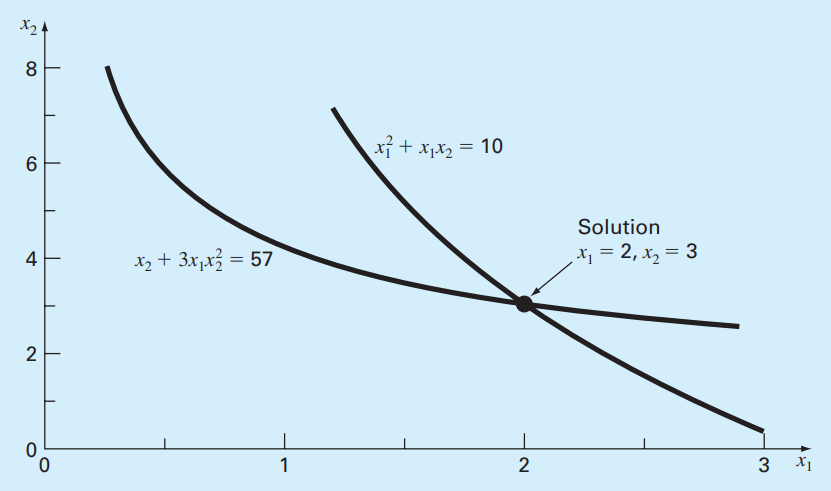
\includegraphics[width=0.75\textwidth]{fig_12_22}
	   \caption{\textsf{a) Graphical depiction of the solution of two simultaneous nonlinear equations.}}
	   \label{fig:fig_12_22}
\end{figure}

Just as we did when we determined roots for single nonlinear equations, such systems
of equations can be expressed generally as

\begin{equation}
f_{1}(x_{1},x_{2},...,x_{n})=0
\end{equation}

\begin{equation}
f_{2}(x_{1},x_{2},...,x_{n})=0
\tag{12.7}
\end{equation}

\begin{equation}
f_{n}(x_{a},x_{2},...,x_{n})=0
\end{equation}

Therefore, the solution are the values of the x's that make the equations equal to zero.

\section*{12.2.1 Successive Substitution}

A simple approach for solving Eq. (12.7) is to use the same strategy that was employed for
fixed-point iteration and the Gauss-Seidel method. That is, each one of the nonlinear equations can be solved for one of the unknowns. These equations can then be implemented
iteratively to compute new values which (hopefully) will converge on the solutions. This
approach, which is called successive substitution, is illustrated in the following example.

\section*{EXAMPLE 12.3 Successive Substitution for a Nonlinear System}

Problem Statement. Use successive substitution to determine the roots of Eq. (12.6).
Note that a correct pair of roots is $x_{1}=2$ and $x_{2}=3$. Initiate the computation with guesses
of $x_{1}=1.5$ and $x_{2}=3.5$.

Solution. Equation (12.6a) can be solved for
\begin{equation}
x_{1}=\frac{10-x^{2}_{1}}{x_{2}}
\tag{E12.2.1}
\end{equation}

and Eq. (12.6b) can be solved for

\begin{equation}
x_{2}=57-3x_{1}x_{2}^{2}
\tag{E12.3.1}
\end{equation}

On the basis of the initial guesses, Eq. (E12.3.1) can be used to determine a new value
of $x_{1}$:
\begin{equation}
x_{1}=\frac{10-(1.5)^{2}}{3.5}=2.21429
\end{equation}

This result and the initial value of $x_{2}=3.5$ can be substituted into Eq. (E12.3.2) to determine a new value of $x_{2}$:

\begin{equation}
x_{2}=57-3(2.21429)(3.5)^{2}=-24.37516
\end{equation}

Thus, the approach seems to be diverging. This behavior is even more pronounced on the
second iteration:

\begin{equation}
x_{1}=\frac{10-(2.21429)^{2}}{-24.37216}=-0.20910
\end{equation}

\begin{equation}
x_{2}=57-3(-0.20910)(-24.37516)^{2}=429.709
\end{equation}


Obviously, the approach is deteriorating.

Now we will repeat the computation but with the original equations set up in a different format. For example, an alternative solution of Eq. (12.6a) is

\begin{equation}
x_{1}=\sqrt{10=x_{1}x_{2}}
\end{equation}

and of Eq. (12.6b) is

\begin{equation}
x_{2}=\sqrt{\frac{57-x_{2}}{3x_{1}}}
\end{equation}

Now the results are more satisfactory:

\begin{equation}
x_{1}=\sqrt{10-1.5(3.5)} = 2.17945
\end{equation}

\begin{equation}
x_{2}=\sqrt{\frac{57-3.5}{3(2.17945)}}=2.86051
\end{equation}

\begin{equation}
x_{1}=\sqrt{10-2.17945(2.86051)}=1.94053
\end{equation}

\begin{equation}
x_{2}=\sqrt{\frac{57-2.86051}{3(1.94053)}}=3.04955
\end{equation}

Thus, the approach is converging on the true values of $x_{1}=2$ and $x_{2}=3$.

The previous example illustrates the most serious shortcoming of successive
substitution—that is, convergence often depends on the manner in which the equations are
formulated. Additionally, even in those instances where convergence is possible, divergence can occur if the initial guesses are insufficiently close to the true solution. These
criteria are so restrictive that fixed-point iteration has limited utility for solving nonlinear
systems.


\section*{12.2.2 Newton-Raphson}

Just as fixed-point iteration can be used to solve systems of nonlinear equations, other open
root location methods such as the Newton-Raphson method can be used for the same purpose. Recall that the Newton-Raphson method was predicated on employing the derivative
(i.e., the slope) of a function to estimate its intercept with the axis of the independent
variable—that is, the root. In Chap. 6, we used a graphical derivation to compute this estimate. An alternative is to derive it from a first-order Taylor series expansion:

\begin{equation}
f(x_{i+1})=f(x_{i})+(x_{i+1}-x_{1})f'(x_{i})
\tag{12.8}
\end{equation}

where xi is the initial guess at the root and $x_{i+1}$ is the point at which the slope intercepts the x axis.
At this intercept, $f(x_{i+1})$ by definition equals zero and Eq. (12.8) can be rearranged to yield

\begin{equation}
x_{i+1}=x_{i}-\frac{f(x_{i})}{f'(x_{i})}
\tag{12.9}
\end{equation}

which is the single-equation form of the Newton-Raphson method.

The multiequation form is derived in an identical fashion. However, a multivariable
Taylor series must be used to account for the fact that more than one independent variable
contributes to the determination of the root. For the two-variable case, a first-order Taylor
series can be written for each nonlinear equation as

\begin{equation}
f_{l,i+1}=f_{l,i}+(x_{l,i+1}-x_{l,i})\frac{\partial f_{l,i}}{\partial x_{1}}+(x_{2,i+1}-x_{2,i})\frac{\partial f_{l,1}}{\partial x_{2}}
\tag{12.10a}
\end{equation}

\begin{equation}
f_{2,i+1}=f_{2,1}+(x_{1,i+1}-x_{l,i})\frac {\partial f_{2,1}}{\partial x_{1}}+(x_{2,i+1}-x_{2,1})\frac{\partial f_{2,1}}{\partial x_{2}}
\tag{12.10b}
\end{equation}

Just as for the single-equation version, the root estimate corresponds to the values of $x_{1}$ and
$x_{2}$, where $s_{1,l+1}$ and $f_{2, i+1}$ equal zero. For this situation, Eq. (12.10) can be rearranged to give

\begin{equation}
\frac{\partial f_{1,i}}{\partial x_{1}}x_{1,i+1}+\frac{\partial f_{1,i}}{\partial x_{2}}x_{2,i+1}=-f_{1,i}+x_{1,i}\frac{\partial f_{1,i}}{\partial x_{1}}+x_{2,i}\frac {\partial f_{1,i}}{\partial x_{2}}
\tag{12.11a}
\end{equation}

\begin{equation}
\frac{\partial f_{2,i}}{\partial x_{1}}x_{1,i+1}+\frac{\partial f_{2,i}}{\partial x_{2}}x_{2,i+1}=-f_{2,i}+x_{1,i}\frac{\partial f_{2,i}}{\partial x_{1}}+x_{2,i}\frac {\partial f_{2,i}}{\partial x_{2}}
\tag{12.11b}
\end{equation}

Because all values subscripted with i's are known (they correspond to the latest guess or
approximation), the only unknowns are $x_{1,i+1}$ and $x_{2,i+1}$. Thus, Eq. (12.11) is a set of
two linear equations with two unknowns. Consequently, algebraic manipulations (e.g.,
Cramer's rule) can be employed to solve for

\begin{equation}
x_{1,i+1}=
x_{1,i}-
\frac{f_{l,1}
\frac{\partial f_{2,i}}{\partial x_{2}}-f_{2,i}\frac{\partial f_{1,i}}{\partial x_{2}}}{\frac{\partial f_{1,i}}{\partial x_{1}}\frac{\partial f_{2,i}}{\partial x_{2}}-\frac{\partial f_{1,i}}{\partial x_{2}}\frac{\partial f_{2,1}}{\partial x_{1}}}
\tag{12.12a}
\end{equation}

\begin{equation}
x_{2.i+1}=x_{2,1-}
\frac{f_{2,i}\frac{\partial f_{1,i} }{\partial x_{1}}-f_{2,i}\frac{\partial f_{2,i}}{\partial x_{1}}}{\frac{\partial f_{1,i}}{\partial x_{1}}\frac{\partial f_{2,i}}{\partial x_{2}}-\frac{\partial f_{1,i}}{\partial x_{2}}\frac{\partial f_{2,i}}{\partial x_{1}}}
\tag{12.12b}
\end{equation}

The denominator of each of these equations is formally referred to as the determinant of the
Jacobian of the system.
Equation (12.12) is the two-equation version of the Newton-Raphson method. As in
the following example, it can be employed iteratively to home in on the roots of two simultaneous equations.

\section*{EXAMPLE 12.4 Newton-Raphson for a Nonlinear System}

Problem Statement. Use the multiple-equation Newton-Raphson method to determine
roots of Eq. (12.6). Initiate the computation with guesses of $x_{1}=1.5$ and $x_{2}=3.5$.
Solution. First compute the partial derivatives and evaluate them at the initial guesses of
x and y:

\begin{equation}
\frac{\partial f_{1,0}}{\partial x_{1}}=2x_{1}+x_{2}=2(1.5)+3.5=6.5
\; \; \; \;
\frac{\partial f_{1,0}}{\partial x_{2}}=x_{1}=1.5
\end{equation}

\begin{equation}
\frac{\partial f_{2,0}}{\partial x_{1}}=3x_{2}^{2}=3(3.5)^{2}=36.75
\; \; \; \; \;
\frac{\partial f_{2,0}}{\partial x_{1}}=1+6x_{1}x_{2}=1+6(1.5)(3.5)=32.5
\end{equation}

Thus, the determinant of the Jacobian for the first iteration is
\begin{equation}
6.5(32.5)-1.5(36.75) = 156.125
\end{equation}

The values of the functions can be evaluated at the initial guesses as

\begin{equation}
f_{1,0}=(1.5)^{2}+1.5(3.5)-10=-2.5
\end{equation}

\begin{equation}
f_{2,0}=3.5+3(1.5)(3.5)^{2}-71=1.625
\end{equation}

These values can be substituted into Eq. (12.12) to give

\begin{equation}
x_{1}=1.5-\frac{-2.5(32.5)-1.625(1.5)}{156.125}=2.03603
\end{equation}

\begin{equation}
x_{2}=3.5-\frac{1.625(6.5)-(-2.5)(36.75}{156.125}== 2.84388
\end{equation}

Thus, the results are converging to the true values of $x_{1}=2$ and $x_{2}=3$. The computation
can be repeated until an acceptable accuracy is obtained.

When the multiequation Newton-Raphson works, it exhibits the same speedy quadratic
convergence as the single-equation version. However, just as with successive substitution,
it can diverge if the initial guesses are not sufficiently close to the true roots. Whereas
graphical methods could be employed to derive good guesses for the single-equation case,
no such simple procedure is available for the multiequation version. Although there are
some advanced approaches for obtaining acceptable first estimates, often the initial guesses
must be obtained on the basis of trial and error and knowledge of the physical system being
modeled.
The two-equation Newton-Raphson approach can be generalized to solve n simultaneous equations. To do this, Eq. (12.11) can be written for the kth equation as

\begin{equation}
\frac{\partial f_{k,i}}{\partial x_{1}}x_{1,i+1}+
\frac{\partial f_{k,i}}{\partial x_{2}}x_{2,i+1}+
\cdots +
\frac{\partial f_{k,i}}{\partial x_{n}}x_{n,i+1}=
-f_{k,i}+
x_{1,i}\frac{\partial f_{k,i}}{\partial x_{1}}+
x_{2,i}\frac{\partial f_{k,i}}{\partial x_{2}}+
\cdots+
x_{n,i}\frac{\partial f_{k,i}}{\partial x_{n}}
\tag{12.13}
\end{equation}

where the first subscript k represents the equation or unknown and the second subscript denotes whether the value or function in question is at the present value (i) or at the next value
(i + 1). Notice that the only unknowns in Eq. (12.13) are the $x_{k,i+1}$ terms on the left-hand
side. All other quantities are located at the present value (i) and, thus, are known at any
iteration. Consequently, the set of equations generally represented by Eq. (12.13) (i.e., with
k = 1, 2,..., n) constitutes a set of linear simultaneous equations that can be solved
numerically by the elimination methods elaborated in previous chapters.
Matrix notation can be employed to express Eq. (12.13) concisely as

\begin{equation}
[J]\{x_{i+1}\}=-\{f\}+[J]\{x_{i}\}
\tag{12.14}
\end{equation}

where the partial derivatives evaluated at i are written as the Jacobian matrix consisting of
the partial derivatives:

\begin{equation}
[J]=\begin{bmatrix}
\frac{\partial f_{1,i}}{\partial x_{1}} &\frac{\partial f_{1,i}}{\partial x_{2}} & \cdots  & \frac{\partial f_{1,i}}{\partial x_{n}}\\
 \frac{\partial f_{2,i}}{\partial x_{1}}& \frac{\partial f_{2,i}}{\partial x_{2}} & \cdots  &\frac{\partial f_{2,i}}{\partial x_{n}} \\
\vdots  &  \vdots &  & \vdots \\
 \frac{\partial f_{n,i}}{\partial x_{1}}& \frac{\partial f_{n,i}}{\partial x_{2}} & \cdots  & \frac{\partial f_{n,i}}{\partial x_{n}}
\end{bmatrix}
\tag{12.15}
\end{equation}

The initial and final values are expressed in vector form as

\begin{equation}
\{x_{1}\}^{T} = \left \lfloor x_{1,i} \; x_{2,i}  \; \cdots \; x_{n,i} \right \rfloor
\end{equation}
and
\begin{equation}
\{x_{i+1}\}^{T}= \left \lfloor x_{1,i+1} \; x_{2,i+1}  \; \cdots \; x_{n,i+1} \right \rfloor
\end{equation}

Finally, the function values at i can be expressed as

\begin{equation}
\{f\}^{T}= \left \lfloor f_{1,i} \; f_{2,i}  \; \cdots \; f_{n,i}\right \rfloor
\end{equation}

Equation (12.14) can be solved using a technique such as Gauss elimination. This
process can be repeated iteratively to obtain refined estimates in a fashion similar to the
two-equation case in Example 12.4.
Insight into the solution can be obtained by solving Eq. (12.14) with matrix inversion.
Recall that the single-equation version of the Newton-Raphson method is

\begin{equation}
x_{i+1}=x_{i}-\frac{f(x_{i})}{f'(x_{1})}
\tag{12.16}
\end{equation}

If Eq. (12.14) is solved by multiplying it by the inverse of the Jacobian, the result is

\begin{equation}
\{x_{i+1}\}=\{x_{i}\}-[J]^{-1}\{f\}
\tag{12.17}
\end{equation}

Comparison of Eqs. (12.16) and (12.17) clearly illustrates the parallels between the
two equations. In essence, the Jacobian is analogous to the derivative of a multivariate
function.
Such matrix calculations can be implemented very efficiently in MATLAB. We can
illustrate this by using MATLAB to duplicate the calculations from Example 12.4. After
defining the initial guesses, we can compute the Jacobian and the function values as

\begin{lstlisting}[numbers=none]
>> x=[1.5;3.5];
>> J=[2*x(1)+x(2) x(1);3*x(2)^2 1+6*x(1)*x(2)]
J =
6.5000 1.5000
36.7500 32.5000
>> f=[x(1)^2+x(1)*x(2)-10;x(2)+3*x(1)*x(2)^2-57]
f =
-2.5000
1.6250
\end{lstlisting}

Then, we can implement Eq. (12.17) to yield the improved estimates

\begin{lstlisting}[numbers=none]
>> x=x-J\f
x =
2.0360
2.8439
\end{lstlisting}

Although we could continue the iterations in the command mode, a nicer alternative is
to express the algorithm as an M-file. As in Fig. 12.4, this routine is passed an M-file that
computes the function values and the Jacobian at a given value of x. It then calls this function and implements Eq. (12.17) in an iterative fashion. The routine iterates until an upper
limit of iterations (maxit) or a specified percent relative error (es) is reached.

\begin{figure}
\begin{lstlisting}[numbers=none]
function [x,f,ea,iter]=newtmult(func,x0,es,maxit,varargin)
% newtmult: Newton-Raphson root zeroes nonlinear systems
% [x,f,ea,iter]=newtmult(func,x0,es,maxit,p1,p2,...):
% uses the Newton-Raphson method to find the roots of
% a system of nonlinear equations
% input:
% func = name of function that returns f and J
% x0 = initial guess
% es = desired percent relative error (default = 0.0001%)
% maxit = maximum allowable iterations (default = 50)
% p1,p2,... = additional parameters used by function
% output:
% x = vector of roots
% f = vector of functions evaluated at roots
% ea = approximate percent relative error (%)
% iter = number of iterations
if nargin<2,error('at least 2 input arguments required'),end
if nargin<3|isempty(es),es=0.0001;end
if nargin<4|isempty(maxit),maxit=50;end
iter = 0;
x=x0;
while (1)
	[J,f]=func(x,varargin{:});
	dx=J\f;
	x=x-dx;
	iter = iter + 1;
	ea=100*max(abs(dx./x));
	if iter>=maxit|ea<=es, break, end
end
\end{lstlisting}
\caption{\textsf{MATLAB M-file to implement Newton-Raphson method for nonlinear systems of equations.}}
\end{figure}

We should note that there are two shortcomings to the foregoing approach. First,
Eq. (12.15) is sometimes inconvenient to evaluate. Therefore, variations of the NewtonRaphson approach have been developed to circumvent this dilemma. As might be expected, most are based on using finite-difference approximations for the partial derivatives
that comprise [J]. The second shortcoming of the multiequation Newton-Raphson method
is that excellent initial guesses are usually required to ensure convergence. Because these
are sometimes difficult or inconvenient to obtain, alternative approaches that are slower
than Newton-Raphson but which have better convergence behavior have been developed.
One approach is to reformulate the nonlinear system as a single function:

\begin{equation}
F(x)=\sum_{i=1}^{n}[f_{i}(x_{1}, x_{2},...,x_{n})]^{2}
\end{equation}

where $f_{i}(x_{1}, x_{2}, ..., x_{n})$ is the ith member of the original system of Eq. (12.7). The values
of x that minimize this function also represent the solution of the nonlinear system. Therefore, nonlinear optimization techniques can be employed to obtain solutions.

\section*{12.3 CASE STUDY CHEMICAL REACTIONS}

Background. Nonlinear systems of equations occur frequently in the characterization
of chemical reactions. For example, the following chemical reactions take place in a closed
system:

\begin{equation}
2A+B\begin{matrix}
\rightarrow \\
\leftarrow
\end{matrix}C
\tag{12.18}
\end{equation}

\begin{equation}
A+D\begin{matrix}
\rightarrow \\
\leftarrow
\end{matrix}C
\tag{12.19}
\end{equation}

At equilibrium, they can be characterized by
\begin{equation}
K_{1}=\frac{c_{c}}{c_{a}^{2}c_{b}}
\tag{12.20}
\end{equation}

\begin{equation}
K_{2}=\frac{c_{x}}{c_{a}x_{d}}
\tag{12.21}
\end{equation}

where the nomenclature ci represents the concentration of constituent i. If x1 and x2 are the
number of moles of C that are produced due to the first and second reactions, respectively,
formulate the equilibrium relationships as a pair of two simultaneous nonlinear equations.
If $K_{1}=4 \times 10^{-4}$, $K_{2}=3.7 \times10^{-2}$, $x_{a,0}=50$, $x_{c,0}=20$, $c_{c,0}=5$ and $c_{d,0}=10$, employ the
Newton-Raphson method to solve these equations.

Solution. Using the stoichiometry of Eqs. (12.18) and (12.19), the concentrations of
each constituent can be represented in terms of $x_{1}$ and $x_{2}$ as

\begin{equation}
c_{a}=c_{a,0}-2x_{1}-x_{2}
\tag{12.22}
\end{equation}

\begin{equation}
c_{b}=c_{b,0}-x_{1}
\tag{12.23}
\end{equation}

\begin{equation}
c_{c}=c_{c,0}+x_{1}+x_{2}
\tag{12.24}
\end{equation}

\begin{equation}
c_{d}=c_{d,0}-x_{2}
\tag{12.25}
\end{equation}

where the subscript 0 designates the initial concentration of each constituent. These values
can be substituted into Eqs. (12.20) and (12.21) to give

\begin{equation}
K_{1}=\frac{(c_{c}+x_{1}+x_{2})}{(c_{a,0}-2x_{x}-x_{2})^{2}(c_{b,0}-x_{1})}
\end{equation}

\begin{equation}
K_{2}=\frac{(c_{c,0}+x_{1}+x_{2})}{(c_{a,0}-2x_{1}-x_{2})()}
\end{equation}

Given the parameter values, these are two nonlinear equations with two unknowns. Thus,
the solution to this problem involves determining the roots of

\begin{equation}
f_{1}(x_{1},x_{2})=\frac{5x+x_{1}+x_{2}}{(50-2x_{2}-x_{2})^{2}(20-x_{1})}-4 \times 10^{-4}
\tag{12.27}
\end{equation}

\begin{equation}
f_{2}(x_{1},x_{2})=\frac{(5+x_{1}+x_{2})}{(50-2x_{1}-x_{2})(10-x_{2})}-3.7 \times10^{-2}
\tag{12.27}
\end{equation}

In order to use Newton-Raphson, we must determine the Jacobian by taking the partial
derivatives of Eqs. (12.26) and (12.27). Although this is certainly possible, evaluating the
derivatives is time consuming. An alternative is to represent them by finite differences in a
fashion similar to the approach used for the modified secant method in Sec. 6.3. For example, the partial derivatives comprising the Jacobian can be evaluated as

\begin{equation}
\frac{\partial f_{1}}{\partial x_{1}}=\frac{f_{1}(x_{1}+\delta x_{1},x_{2})-f_{1}(x_{1},x_{2})}{\delta x_{1}}
\; \; \; \; \; \; \; \; \; \;
\frac{\partial f_{1}}{\partial x_{2}}=\frac{f_{1}(x_{1}, x_{2}+\delta x_{2})-f_{1}(x_{1},x_{2})}{\delta x_{2}}
\end{equation}

\begin{equation}
\frac{\partial f_{2}}{\partial x_{1}}=\frac{f_{2}(x_{1}+\delta x_{1},x_{2})-f_{2}(x_{1},x_{2})}{\delta x_{1}}
\; \; \; \; \; \; \; \; \; \;
\frac{\partial f_{2}}{\partial x_{2}}=\frac{f_{2}(x_{1}, x_{2}+\delta x_{2})-f_{2}(x_{1},x_{2})}{\delta x_{2}}
\end{equation}

These relationships can then be expressed as an M-file to compute both the function
values and the Jacobian as

\begin{lstlisting}[numbers=none]
function [J,f]=jfreact(x,varargin)
del=0.000001;
df1dx1=(u(x(1)+del*x(1),x(2))-u(x(1),x(2)))/(del*x(1));
df1dx2=(u(x(1),x(2)+del*x(2))-u(x(1),x(2)))/(del*x(2));
df2dx1=(v(x(1)+del*x(1),x(2))-v(x(1),x(2)))/(del*x(1));
df2dx2=(v(x(1),x(2)+del*x(2))-v(x(1),x(2)))/(del*x(2));
J=[df1dx1 df1dx2;df2dx1 df2dx2];
f1=u(x(1),x(2));
f2=v(x(1),x(2));
f=[f1;f2];
function f=u(x,y)
f = (5 + x + y) / (50 - 2 * x - y) ^ 2 / (20 - x) - 0.0004;
function f=v(x,y)
f = (5 + x + y) / (50 - 2 * x - y) / (10 - y) - 0.037;
\end{lstlisting}

The function newtmult (Fig. 12.4) can then be employed to determine the roots given initial guesses of x1 = x2 = 3:
\begin{lstlisting}[numbers=none]
>> format short e
>> [x,f,ea,iter]=newtmult(@jfreact,x0)
x =
	3.3366e+000
	2.6772e+000
f =
	-7.1286e-017
		8.5973e-014
ea =
		5.2237e-010
iter =
		4
\end{lstlisting}

After four iterations, a solution of $x_{1}=3.3366$ and $x_{2}=2.6772$ is obtained. These values
can then be substituted into Eq. (12.22) through (12.25) to compute the equilibrium concentrations of the four constituents:

\begin{equation}
c_{a}=50-2(3.3366)-2.6772=40.6496
\end{equation}

\begin{equation}
c_{b}=20-3.3366=12.6634
\end{equation}

\begin{equation}
c_{c}=5+3.3366+2.6772=11.0138
\end{equation}

\begin{equation}
c_{d}=10-2.6772=7.3228
\end{equation}



STRONA PODWÓJNA - 320
12.1 Solve the following system using three iterations with
Gauss-Seidel using overrelaxation ($\lambda =1.25$). If necessary,
rearrange the equations and show all the steps in your solution including your error estimates. At the end of the computation, compute the true error of your final results.

\begin{equation}
3x_{1}+8_{2}=11
\end{equation}

\begin{equation}
6x_{1}-x_{2}=5
\end{equation}

12.2 (a) Use the Gauss-Seidel method to solve the following
system until the percent relative error falls below $\varepsilon_{s}=5\%$:

\begin{equation}
\begin{bmatrix}
0.8 & -0.4 & \\
-0.4 & 0.8 & -0.4\\
 & -0.4 & 0.8
\end{bmatrix} \begin{Bmatrix}
x_{1}\\
x_{2}\\
x_{3}
\end{Bmatrix}=\begin{Bmatrix}
41\\
25\\
105
\end{Bmatrix}
\end{equation}

b) Repeat (a) but use overrelaxation with $\lambda =1.2$.

12.3 Use the Gauss-Seidel method to solve the following
system until the percent relative error falls below $\varepsilon_{s} = 5\%$:

\begin{equation}
20x_{1}+2x_{2}-x_{3}=27
\end{equation}

\begin{equation}
-3x_{1}-6x_{2}+2x_{3}=-61.5
\end{equation}

\begin{equation}
x_{1}+x_{2}+5x_{3}=-21.5
\end{equation}

12.4 Repeat Prob. 12.3 but use Jacobi iteration.
12.5 The following system of equations is designed to determine concentrations (the c's in g/m3
) in a series of coupled
reactors as a function of the amount of mass input to each
reactor (the right-hand sides in g/day):

\begin{equation}
15c_{1}-3c_{2}-c_{3}=3800
\end{equation}

\begin{equation}
-3c_{1}+18c_{2}-6c_{3}=1200
\end{equation}


\begin{equation}
-4c_{1}-c_{2}+12c_{3}=2350
\end{equation}

\begin{figure}[H]
		\centering
		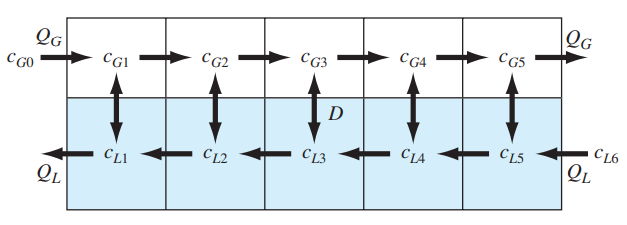
\includegraphics[width=0.75\textwidth]{fig_12_23}
	   \label{fig:fig_12_23}
\end{figure}

Solve this problem with the Gauss-Seidel method to $\varepsilon _{s}=5\%$.
12.6 Use the Gauss-Seidel method (a) without relaxation
and (b) with relaxation ($\lambda =1.2$) to solve the following system to a tolerance of $\varepsilon _{s}=5\%$. If necessary, rearrange the
equations to achieve convergence.

\begin{equation}
2x_{2}-6x_{2}-x_{3}=-38
\end{equation}

\begin{equation}
-3x_{1}-x_{2}+7x_{3}=-34
\end{equation}

\begin{equation}
-8x_{1}+x_{2}-2x_{3}=-20
\end{equation}

12.7 Of the following three sets of linear equations, identify
the set(s) that you could not solve using an iterative method
such as Gauss-Seidel. Show using any number of iterations
that is necessary that your solution does not converge.
Clearly state your convergence criteria (how you know it is
not converging).

\begin{figure}[H]
		\centering
		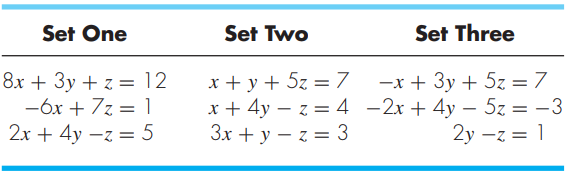
\includegraphics[width=0.75\textwidth]{fig_12_24}
	   \label{fig:fig_12_24}
\end{figure}

12.8 Determine the solution of the simultaneous nonlinear
equations
\begin{equation}
y=-x^{2}+x+0.5
\end{equation}

\begin{equation}
y+5xy=x^{2}
\end{equation}

Use the Newton-Raphson method and employ initial guesses
of $x=y=1.2$.
12.9 Determine the solution of the simultaneous nonlinear
equations:

\begin{equation}
x^{2}=5-y^{2}
\end{equation}

\begin{equation}
y+1=x^{2}
\end{equation}

(a) Graphically.
(b) Successive substitution using initial guesses of $x=y=1.5$.
(c) Newton-Raphson using initial guesses of $x=y=1.5$.

12.10 Figure P12.10 depicts a chemical exchange process
consisting of a series of reactors in which a gas flowing
from left to right is passed over a liquid flowing from right
to left. The transfer of a chemical from the gas into the
liquid occurs at a rate that is proportional to the difference
between the gas and liquid concentrations in each reactor.
At steady state, a mass balance for the first reactor can be
written for the gas as

\begin{equation}
Q_{G^{C}G0}-Q_{G^{C}G1}+D_{(C_{L1}-C_{G1})}
\end{equation}

and for the liquid as
\begin{equation}
Q_{L^{C}L2}-Q_{L^{C}L1}+D(C_{G1}-C_{L1})=0
\end{equation}

where QG and QL are the gas and liquid flow rates, respectively, and D = the gas-liquid exchange rate. Similar balances
can be written for the other reactors. Use Gauss-Seidel without relaxation to solve for the concentrations given the following values: $Q_{G}=2$,$Q_{L}=1$, D = 0.8, $c_{G0}=100$, $c_{L}6$.

12.11 The steady-state distribution of temperature on a
heated plate can be modeled by the Laplace equation:

\begin{equation}
0=\frac{\partial^2 T}{\partial x^2}+\frac{\partial^2 T}{\partial y^2}
\end{equation}


If the plate is represented by a series of nodes (Fig. P12.11),
centered finite differences can be substituted for the second
derivatives, which result in a system of linear algebraic
equations. Use the Gauss-Seidel method to solve for the
temperatures of the nodes in Fig. P12.11.
12.12 Develop your own M-file function for the GaussSeidel method without relaxation based on Fig. 12.2, but

\begin{figure}[H]
		\centering
		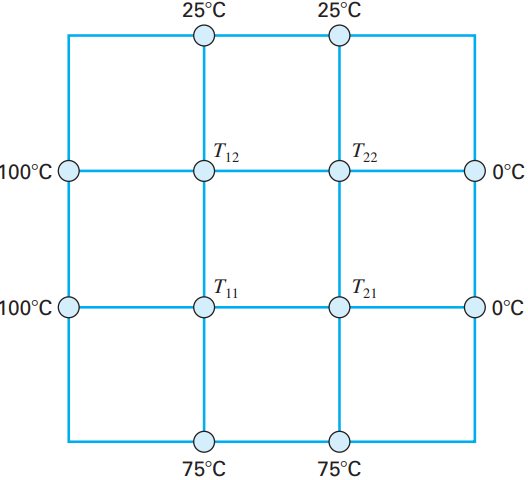
\includegraphics[width=0.75\textwidth]{fig_12_25}
	   \label{fig:fig_12_25}
\end{figure}

change the first line so that it returns the approximate error
and the number of iterations:

\begin{lstlisting}[numbers=none]
function [x,ea,iter] = ...
	GaussSeidel(A,b,es, maxit)
\end{lstlisting}

Test it by duplicating Example 12.1 and then use it to solve
Prob. 12.2a.
12.13 Develop your own M-file function for Gauss-Seidel
with relaxation. Here is the function's first line:

\begin{lstlisting}[numbers=none]
function [x,ea,iter] = ...
	GaussSeidelR(A,b,lambda,es,maxit)
\end{lstlisting}

In the event that the user does not enter a value for $\lambda$, set the
default value as $\lambda=1$.Test it by duplicating Example 12.2
and then use it to solve Prob. 12.2b.
12.14 Develop your own M-file function for the NewtonRaphson method for nonlinear systems of equations based
on Fig. 12.4. Test it by solving Example 12.4 and then use it
to solve Prob. 12.8.

\end{document}
